% 2008 年江西卷文科第 16 题：正六边形 ABCDEF 及由 A 引出的对角线。
% 来源 PDF：gaokaomath-src/普通高考/2008/2008江西文.pdf
% SHA-256：8505b08b95152dbb1421e3f2d72c379b24c8ab6cb47bcc1dbdc8feb058459cda
% 原页：2008江西文.pdf 第 1 页（A3 三栏）第 2 栏，书页码 461。
% 绘制依据：按原页顶点次序 A（下）、B（右下）、C（右）、D（右上）、E（左上）、F（左），
%   并画出由 A 引出的对角线 AC、AD、AE 与边 AF。
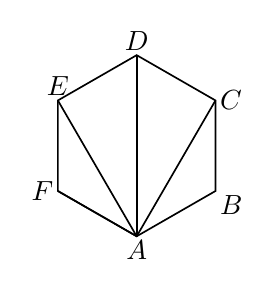
\begin{tikzpicture}[scale=1.15, semithick, every node/.style={inner sep=1.4pt}]
  \coordinate (A) at (0.00,-1.00);
  \coordinate (B) at (0.87,-0.50);
  \coordinate (C) at (0.87,0.50);
  \coordinate (D) at (0.00,1.00);
  \coordinate (E) at (-0.87,0.50);
  \coordinate (F) at (-0.87,-0.50);

  \draw (A) -- (B) -- (C) -- (D) -- (E) -- (F) -- cycle;
  \draw (A) -- (C);
  \draw (A) -- (D);
  \draw (A) -- (E);
  \draw (A) -- (F);

  \node[below] at (A) {$A$};
  \node[below right] at (B) {$B$};
  \node[right] at (C) {$C$};
  \node[above] at (D) {$D$};
  \node[above] at (E) {$E$};
  \node[left] at (F) {$F$};
\end{tikzpicture}
